\documentclass[border=4pt]{standalone}
\usepackage{fontspec}
\usepackage{amsmath}
\usepackage{unicode-math}
\setmainfont{Latin Modern Roman}
\setmathfont{Latin Modern Math}
\usepackage{pgfplots}
\usepackage{pgfplotstable}
\pgfplotsset{compat=1.18}
\usepackage{tkz-euclide}
\usetikzlibrary{arrows.meta,calc,angles,quotes,patterns,3d,backgrounds}
\definecolor{ink}{HTML}{123428}
\definecolor{asy}{HTML}{475569}
\definecolor{mint}{HTML}{86e0bd}
\tikzset{asym/.style={asy, line width=0.9pt, dash pattern=on 5pt off 3.5pt},
         guide/.style={gray!70, line width=0.6pt, densely dotted},
         dot/.style={circle, inner sep=0pt, minimum size=5pt, draw=white, line width=0.5pt},
         odot/.style={circle, inner sep=0pt, minimum size=5.5pt, fill=white, line width=1pt},
         lab/.style={font=\footnotesize, inner sep=1.5pt, text=ink}}
\begin{document}
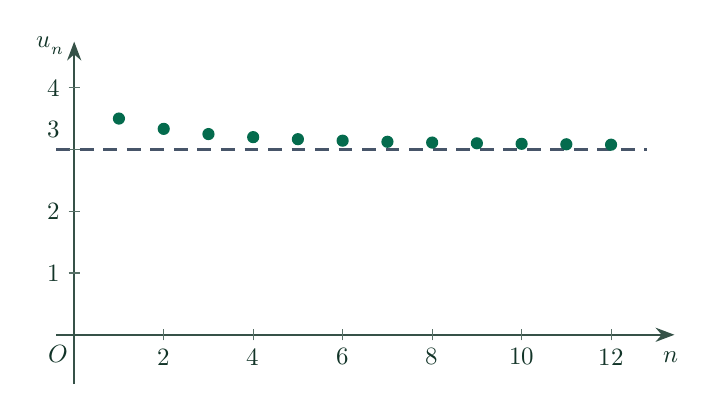
\begin{tikzpicture}
\draw[ink!85, line width=0.7pt, -{Stealth[length=2.4mm]}] (0.000,0.627) -- (7.850,0.627);
\draw[ink!85, line width=0.7pt, -{Stealth[length=2.4mm]}] (0.227,0.000) -- (0.227,4.350);
\draw[asy, line width=0.8pt, dash pattern=on 5pt off 3.5pt] (0.000,2.980) -- (7.500,2.980);
\fill[color={rgb,255:red,4;green,107;blue,77}] (0.795,3.373) circle (2.2pt);
\fill[color={rgb,255:red,4;green,107;blue,77}] (1.364,3.242) circle (2.2pt);
\fill[color={rgb,255:red,4;green,107;blue,77}] (1.932,3.176) circle (2.2pt);
\fill[color={rgb,255:red,4;green,107;blue,77}] (2.500,3.137) circle (2.2pt);
\fill[color={rgb,255:red,4;green,107;blue,77}] (3.068,3.111) circle (2.2pt);
\fill[color={rgb,255:red,4;green,107;blue,77}] (3.636,3.092) circle (2.2pt);
\fill[color={rgb,255:red,4;green,107;blue,77}] (4.205,3.078) circle (2.2pt);
\fill[color={rgb,255:red,4;green,107;blue,77}] (4.773,3.068) circle (2.2pt);
\fill[color={rgb,255:red,4;green,107;blue,77}] (5.341,3.059) circle (2.2pt);
\fill[color={rgb,255:red,4;green,107;blue,77}] (5.909,3.052) circle (2.2pt);
\fill[color={rgb,255:red,4;green,107;blue,77}] (6.477,3.046) circle (2.2pt);
\fill[color={rgb,255:red,4;green,107;blue,77}] (7.045,3.041) circle (2.2pt);
\draw[ink!70] (1.364,0.557) -- (1.364,0.697);
\draw[ink!70] (2.500,0.557) -- (2.500,0.697);
\draw[ink!70] (3.636,0.557) -- (3.636,0.697);
\draw[ink!70] (4.773,0.557) -- (4.773,0.697);
\draw[ink!70] (5.909,0.557) -- (5.909,0.697);
\draw[ink!70] (7.045,0.557) -- (7.045,0.697);
\draw[ink!70] (0.157,1.412) -- (0.297,1.412);
\draw[ink!70] (0.157,2.196) -- (0.297,2.196);
\draw[ink!70] (0.157,2.980) -- (0.297,2.980);
\draw[ink!70] (0.157,3.765) -- (0.297,3.765);
\node[font=\small, text=ink] at (7.800,0.347) {$n$};
\node[font=\small, text=ink] at (-0.073,4.300) {$u_n$};
\node[font=\small, text=ink, inner sep=0.5pt, fill=white] at (1.364,0.347) {$2$};
\node[font=\small, text=ink, inner sep=0.5pt, fill=white] at (2.500,0.347) {$4$};
\node[font=\small, text=ink, inner sep=0.5pt, fill=white] at (3.636,0.347) {$6$};
\node[font=\small, text=ink, inner sep=0.5pt, fill=white] at (4.773,0.347) {$8$};
\node[font=\small, text=ink, inner sep=0.5pt, fill=white] at (5.909,0.347) {$10$};
\node[font=\small, text=ink, inner sep=0.5pt, fill=white] at (7.045,0.347) {$12$};
\node[font=\small, text=ink, inner sep=0.5pt, fill=white] at (-0.028,1.412) {$1$};
\node[font=\small, text=ink, inner sep=0.5pt, fill=white] at (-0.028,2.196) {$2$};
\node[font=\small, text=ink, inner sep=0.5pt, fill=white] at (-0.028,3.240) {$3$};
\node[font=\small, text=ink, inner sep=0.5pt, fill=white] at (-0.028,3.765) {$4$};
\node[font=\small, text=ink, inner sep=0.5pt] at (0.027,0.387) {$O$};
\end{tikzpicture}
\end{document}
